\documentclass[tikz,border=2pt,11pt]{standalone}
\usetikzlibrary{positioning}
\usetikzlibrary{arrows.meta}
\usetikzlibrary{patterns}
\usetikzlibrary{calc}
\usetikzlibrary{fit}
\usetikzlibrary{decorations.pathreplacing}
\usepackage{amsmath}
\usepackage{amssymb}
\usepackage{bm}
\usepackage{graphicx}
\usepackage{xcolor}
\usepackage{tikz}
\newcommand{\R}{\mathbb R}
\newcommand{\C}{\mathbb C}
\newcommand{\N}{\mathbb N}
\newcommand{\Z}{\mathbb Z}
\newcommand{\E}{\mathbb E}
\newcommand{\dd}{\,\mathrm d}
\newcommand{\one}{\mathbf 1}
\DeclareMathOperator{\Lip}{Lip}
\DeclareMathOperator{\supp}{supp}
\DeclareMathOperator{\dist}{dist}
\newcommand{\norm}[1]{\left\|#1\right\|}
\newcommand{\abs}[1]{\left|#1\right|}
\begin{document}
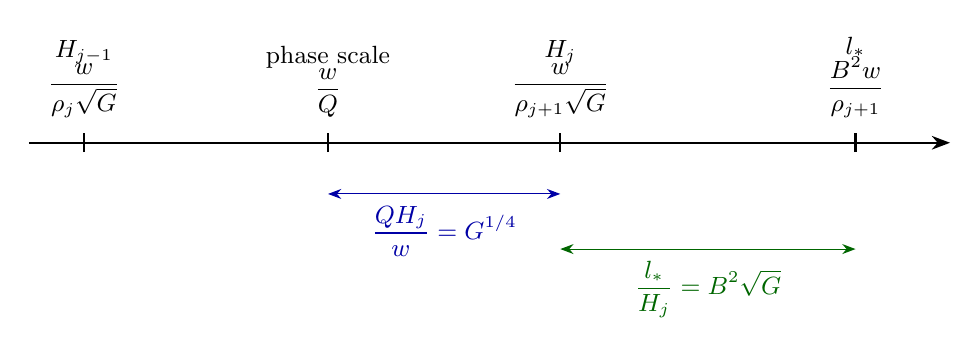
\begin{tikzpicture}[x=1cm,y=1cm,font=\small,>=Stealth]
 \draw[->,thick] (0,0)--(11.7,0);
 \foreach \xx in {.7,3.8,6.75,10.5}
   \draw[thick] (\xx,-.12)--(\xx,.12);
 \node[above,align=center] at (.7,.2)
   {\(H_{j-1}\)\\[-1pt]\(\displaystyle\frac{w}{\rho_j\sqrt G}\)};
 \node[above,align=center] at (3.8,.2)
   {phase scale\\[-1pt]\(\displaystyle\frac{w}{Q}\)};
 \node[above,align=center] at (6.75,.2)
   {\(H_j\)\\[-1pt]\(\displaystyle\frac{w}{\rho_{j+1}\sqrt G}\)};
 \node[above,align=center] at (10.5,.2)
   {\(l_*\)\\[-1pt]\(\displaystyle\frac{B^2w}{\rho_{j+1}}\)};
 \draw[<->,blue!65!black] (3.8,-.65)--(6.75,-.65);
 \node[below,blue!65!black] at (5.275,-.68)
   {\(\displaystyle\frac{QH_j}{w}=G^{1/4}\)};
 \draw[<->,green!40!black] (6.75,-1.35)--(10.5,-1.35);
 \node[below,green!40!black] at (8.625,-1.38)
   {\(\displaystyle\frac{l_*}{H_j}=B^2\sqrt G\)};
\end{tikzpicture}
\end{document}
